\chapter{Proposed approach}\label{proposed_approach}

\section{Aim}

This project aims to improve the experience of using Google Drive specifically for power users. Regular users can benefit from it as well -- provided they follow some prerequisite steps in order to use the application.

If successful, it will drastically diminish the some of the issues described in section~\ref{main_disadvantages}.

\section{Summary}

In essence, Google Drive is nothing more than a remote storage system. All the operations that a user might want to execute on a local storage system (e.g. copying files, creating and organising directories, reading and writing data) have an equivalent operation on Google Drive.

Disk-based storage devices are organized by the operating system using a file system in order to keep track of all the data they contain. This happens behind the scences. Users can interact with the storage device using system calls. Some of the more popular ones are \codeword{read}, \codeword{write}, \codeword{close}, \codeword{wait}, \codeword{exec}, \codeword{fork}, \codeword{exit}, \codeword{kill}. Note that not all of these deal with file storage. Some of them are a proxy which expose different functionalities of the operating system. In addition, users seldom execute system calls manually. It is the task of higher level applications to do this instead.

An interesting concept comes to mind: why not model a Google Drive account in such a way that it behaves identically to a traditional file system? The only difference would be that instead of storing and reading data from a local disk, it would interact with Google's servers.

GCSF does exactly that. It is a virtual file system on top of Google Drive. It allows users to mount their Drive account locally and interact with it as they would with a regular disk partition. This is achieved using the FUSE (Filesystem in Userspace) interface~\cite{libfuse}, as described in section \ref{implementation}.

\section{Usage}

Before delving into implementation details, I present a brief overview of how GCSF works from the user perspective.

GCSF consists of a single binary. When executed with no arguments, it prints a help menu as seen in listing \ref{gcsf_help_menu}. Users can choose to mount the file system to a local directory. GCSF points to an authentication URL (listing~\ref{gcsf_mount}) that must be accessed in order to authorize access to Google Drive (fig.~\ref{fig:drive_auth}). Upon completing the authentication process, GCSF mounts the file system and populates it with all files and directories contained in the \emph{My Drive} directory on Google Drive. This can be observed using tools such as \codeword{df} (listing~\ref{df_output}) and \codeword{mount} (listing~\ref{mount_output}).

\begin{lstlisting}[basicstyle=\footnotesize\ttfamily,caption=GCSF help menu,frame=single,label=gcsf_help_menu,float]
$ gcsf
GCSF 0.1.3
Sergiu Puscas <srg.pscs@gmail.com>
Filesystem based on Google Drive

USAGE:
    gcsf <SUBCOMMAND>

FLAGS:
    -h, --help       Prints help information
    -V, --version    Prints version information

SUBCOMMANDS:
    help      Prints this message or the help of the given subcommand(s)
    logout    Delete credentials file
    mount     Mount the filesystem
\end{lstlisting}

\begin{lstlisting}[basicstyle=\footnotesize\ttfamily,caption=GCSF mount,frame=single,label=gcsf_mount,float]
$ gcsf mount /mnt/gcsf
Please direct your browser to https://accounts.google.com/o/oauth2/[...] and follow the instructions displayed there.
\end{lstlisting}

\begin{figure}[bpt]
\centering
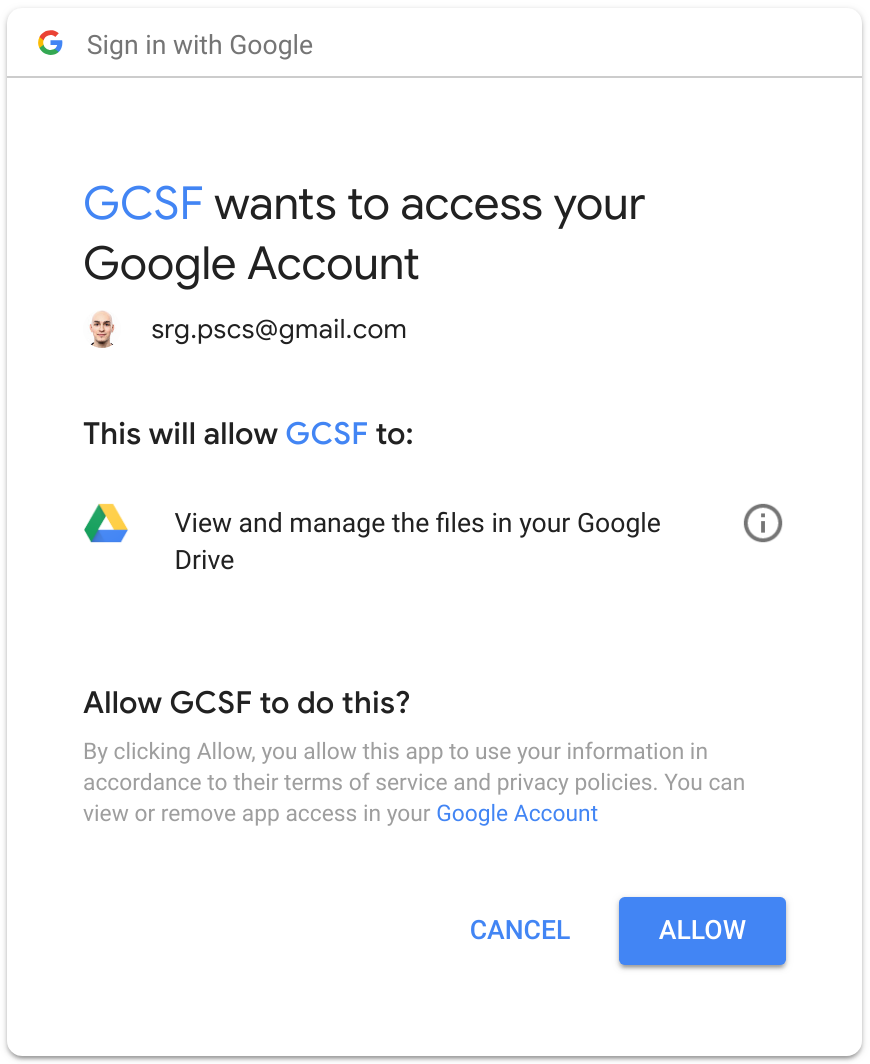
\includegraphics[width=0.7\textwidth]{gcsf_auth}
\caption{Google Drive authorization}
\label{fig:drive_auth}
\end{figure}

\begin{lstlisting}[basicstyle=\footnotesize\ttfamily,caption=Size and capacity of mounted filesystems,frame=single,label=df_output,float]
$ df -h
Filesystem      Size  Used Avail Use% Mounted on
/dev/nvme0n1p5   64G   45G   17G  74% /
/dev/nvme0n1p6  644G  559G   53G  92% /home
/dev/nvme0n1p1  256M   73M  184M  29% /boot
GCSF             15G   11G  4.6G  70% /mnt/gcsf
\end{lstlisting}

\begin{lstlisting}[basicstyle=\footnotesize\ttfamily,caption=Output of mount,frame=single,label=mount_output,float]
$ mount | grep GCSF
GCSF on /mnt/gcsf type fuse (rw,nosuid,nodev,relatime,user_id=1000,group_id=100,allow_other)
\end{lstlisting}


Now the mount directory can be accessed using a file explorer such as \emph{Ranger} (fig.~\ref{fig:ranger}) or \emph{Thunar} (fig.~\ref{fig:thunar}). Command line programs such as \codeword{ls} or \codeword{exa} work as well (fig.~\ref{fig:ls}). From this point onward, the mount directory can be treated as a regular local directory apart from a few exceptions.

\begin{figure}[tbp]
\caption{Ranger window}
\label{fig:ranger}
\centering
\fbox{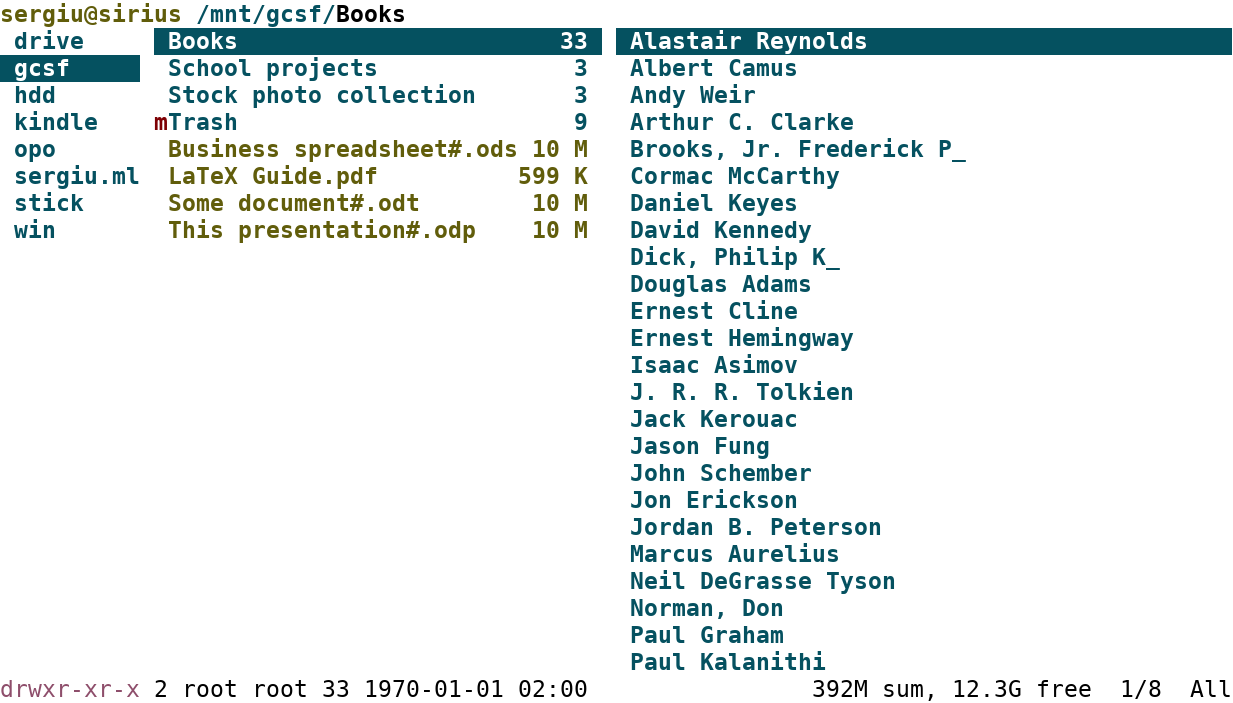
\includegraphics[width=\textwidth]{ranger_white}}
\end{figure}

\begin{figure}[tbp]
\caption{Thunar window}
\label{fig:thunar}
\centering
\fbox{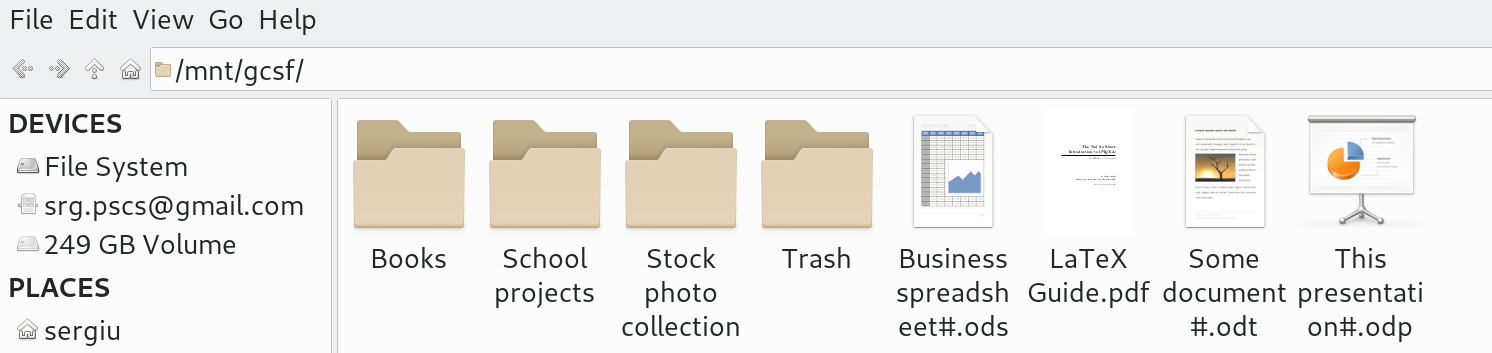
\includegraphics[width=\textwidth]{thunar}}
\end{figure}

\begin{figure}[tbp]
  \caption{File listing}
\label{fig:ls}
\centering
\fbox{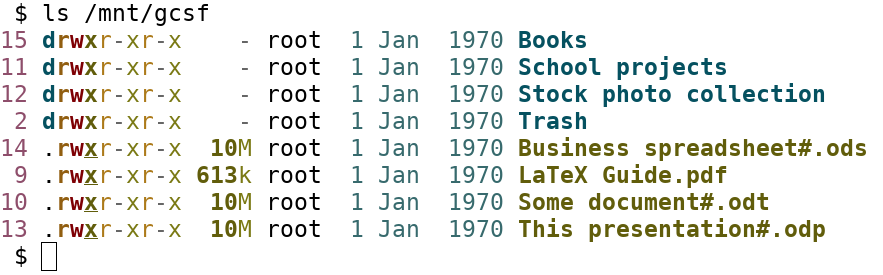
\includegraphics[width=\textwidth]{ls_white}}
\end{figure}

\subsection{Exceptions}

As can be seen in fig.~\ref{fig:ls}, some files have a \codeword{#} symbol attached at the end of their name. This is the case for special Google Drive files, including spreadsheets, docs and slides. Since their file format and size is undefined at this point, GCSF reports the maximum file size supported for these types of files. When such a file is accessed by a user, GCSF chooses the most appropriate filetype and exports the file from Drive. It also adds the appropriate extension to the file name and updates its real size (fig.~\ref{fig:export_doc}). Due to the nature of such files, they cannot be edited locally and are essentially limited to read-only access. However, they can be exported in a known file format, edited locally and then stored separately using GCSF.

\begin{figure}[tbp]
\caption{Exporting Google Docs as OpenDocument files.}
\label{fig:export_doc}
\centering
\fbox{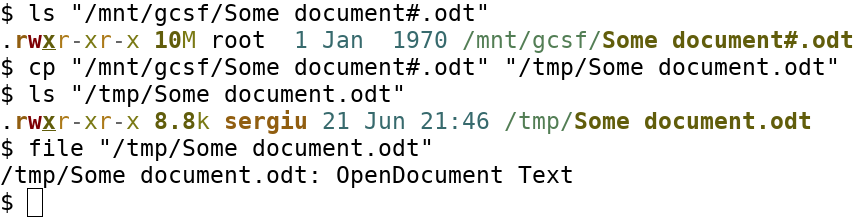
\includegraphics[width=\textwidth]{export_white}}
\end{figure}


\section{Implementation} \label{implementation}

\subsection{Rust}

Rust is a relatively new systems programming language sponsored by the Mozilla Foundation~\cite{rust_website}. According to \emph{The Rust Programming Language} book~\cite{trpl},

\begin{quote}
Rust is a programming language that helps you write faster, more reliable software. High-level ergonomics and low-level control are often at odds with each other in programming language design; Rust stands to challenge that. Through balancing powerful technical capacity and a great developer experience, Rust gives you the option to control low-level details (such as memory usage) without all the hassle traditionally associated with such control.
\end{quote}

From this description, Rust seems like a good fit for this type of project. However, there are a few specific reasons why I chose it instead of a different language:

\begin{enumerate}
  \itemsep0em
  \item Performance. Rust is in many cases on par with C/C++ (or even faster!) in terms of performance~\cite{rust_vs_cpp_benchmark}. Compared to interpreted languages like Python or Ruby, this is a clear advantage.
  \item Type safety. Any code that may lead to undefined behavior in Rust must be explicitly wrapped within an \codeword{unsafe { }} block, making it the programmer's responsibility to make sure that the code is correct. GCSF does not contain unsafe blocks.
  \item Memory safety.
    \begin{itemize}
      \itemsep0em
      \item \emph{No null pointer dereferences}. Rust does not have the concept of a \codeword{NULL} pointer. Instead, it uses a construct borrowed from the functional world (\codeword{Option<T>}) which encourages the programmer to always check the existence of a packed value.
      \item \emph{No dangling pointers}. Instead of using a garbage collector, Rust has a set of rules that define when and how allocated memory is freed. All of these rules are enforced at compile time, thus eliminating an entire category of runtime errors. The rules are:
      \begin{enumerate}
        \itemsep0em
        \item Any value has a single owner at any given time.
        \item References can not outlive the objects they point to.
        \item At any point, there can be at most one mutable reference \emph{or} any number of immutable (read-only) references to a value.
      \end{enumerate}
      \item \emph{No buffer overruns.}
    \end{itemize}
  \item Easy integration of third-party libraries using the \codeword{cargo} package manager and the official package registry~\cite{crates_io}.
  \item Support for the functional paradigm. Rust uses many functional concepts, \emph{closures} and \emph{iterators} being two notable examples.
  \item Standardized ecosystem and builtin tools. Rust packages are commonly published on \url{crates.io}~\cite{crates_io}. Documentation is generated by \codeword{rustdoc} and published automatically to \url{docs.rs}~\cite{docs_rs}. The official style guide can be enforced using \codeword{rustfmt}.
  \item Community and growth. According to the \emph{stackoverflow developer survey}~\cite{stack_overflow_most_loved}, developers have chosen Rust as the most loved programming language for three years in a row.
\end{enumerate}

Some of the points stated above are discussed in more depth in Jim Blandy's book \emph{Why Rust?}~\cite{why_rust}.

\subsection{FUSE}

FUSE (\textbf{F}ilesystem in \textbf{Use}rspace) is a project that allows users to create virtual filesystems in the user level. Internally, it delegates tasks to a kernel module. As a result, users do not have to interact with the kernel directly. FUSE is a popular choice for esoteric filesystems which do not store data themselves. A few notable examples are \emph{sshfs}~\cite{sshfs}, which mounts a remote filesystem using SFTP~\cite{sftp}, and \emph{WikipediaFS}~\cite{wikipediafs} which allows users to view and edit articles locally.

FUSE is made up of two components:
\begin{itemize}
  \itemsep0em
  \item the \textit{fuse} kernel module
  \item the \textit{libfuse} userspace library
\end{itemize}

FUSE filesystems are usually implemented as regular applications that interact with the \textit{libfuse} library. This library provides two interfaces that are useful for defining the behavior of the filesystem. In both cases, the filesystem receives incoming requests from the kernel, which are provided as calls to methods defined in the interface.

% First, there is the high-level interface (appendix~\ref{appendix:fuse_high_level}). It uses high-level concepts such as file names and paths in most of its methods. Second, there is the low-level interface (appendix~\ref{appendix:fuse_low_level}). Files are identified using low level concepts such as inodes~\cite{tanenbaum}. GCSF uses the latter because of the available language library for Rust, provided through the \codeword{fuse} crate~\cite{fuse_crate}. GCSF implements the \codeword{Filesystem} trait defined in appendix~\ref{appendix:rust_fuse}.
First, there is the high-level interface. It uses concepts such as file names and paths in most of its methods. Second, there is the low-level interface, which uses inodes in order to identify files~\cite{tanenbaum}. GCSF uses the latter because of the available language library for Rust, provided through the \codeword{fuse} crate~\cite{fuse_crate}. GCSF implements the \codeword{Filesystem} trait defined in appendix~\ref{appendix:rust_fuse}.

\subsection{Drive API}

Google provides a REST API for interacting with Drive~\cite{google_drive_rest_api_overview}. It also provides official client libraries for multiple programming languages: Java, Javascript, .NET, Objective-C, PHP and Python. There are also early-stage libraries for Dart, Go, Node.js and Ruby.

Unfortunately, Rust is not officially supported. There is however a set of unofficial libraries, programatically generated by Sebastian Thiel~\cite{google_apis_rs,sebastian_thiel}. Although imperfect, they are good enough for the scope of this project. Some limitations are described in section \ref{problems_encountered}.

\subsection{Architecture}

The heart of the application is the \codeword{GCSF} struct. It implements the \codeword{Filesystem} trait from the \codeword{fuse} module, essentially making it a mountable file system. Internally, a \codeword{FileManager} is used for bookkeeping. The \codeword{FileManager} provides all the required functionality for dealing with local files and directories. It keeps track of the file hierarchy, inodes, metadata and performs regular syncs. In order to communicate with Drive, it uses a \codeword{DriveFacade} which facilitates remote operations. The \codeword{DriveFacade} is linked to the user's account.

These abstractions create a distinct separation of responsibilities. For instance, anything that requires network communication is performed by the \codeword{DriveFacade}. Information about any file can be obtained by simply querying the \codeword{FileManager}. (Un)mounting the file system and responding to system calls is done by \codeword{GCSF}.

Figure \ref{fig:gcsf_architecture} outlines how these components interact with each other.

\begin{figure}[bpt]
\caption{GCSF architecture}
\label{fig:gcsf_architecture}
\centering
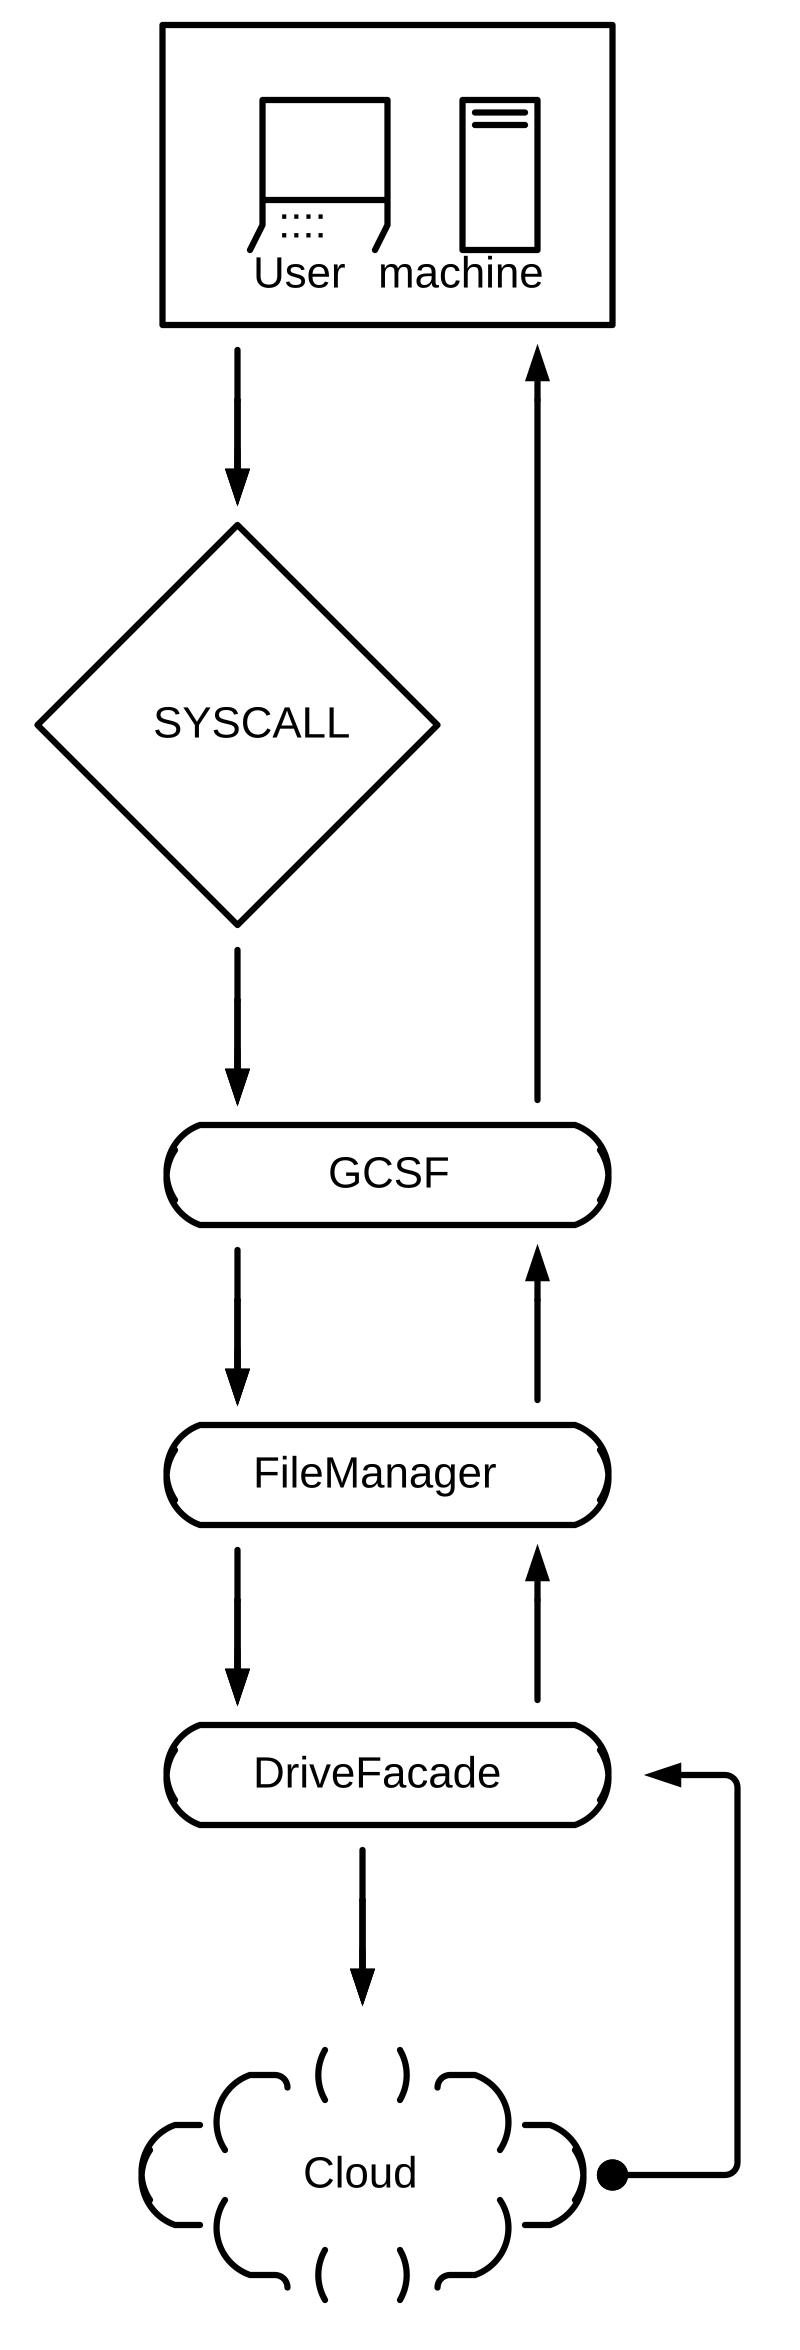
\includegraphics[width=0.4\linewidth]{gcsf_architecture}
\end{figure}

\subsection{Configuration}

A configuration file can be used in order to set different parameters for GCSF. One example can be found in listing \ref{gcsf_config}. 

\begin{lstlisting}[basicstyle=\footnotesize\ttfamily,caption=GCSF configuration file, frame=single, label=gcsf_config,float]
### This is the configuration file that GCSF uses.
### It should be placed in $XDG_CONFIG_HOME/gcsf/gcsf.toml,
### which is usually defined as $HOME/.config/gcsf/gcsf.toml

# Show debug logs?
debug = true

# How long to cache the contents of a file after it has been
# accessed.
cache_max_seconds = 300

# How how many files to cache.
cache_max_items = 10

# How long to cache the size and capacity of the filesystem.
# These are the values reported by `df'.
cache_statfs_seconds = 1

# How many seconds to wait before checking for remote changes
# and updating them locally.
sync_interval = 10000

# Mount options
mount_options = [
    "fsname=GCSF",
    "allow_root",
    "big_writes",
    "max_write=131072"
]

# If set to true, Google Drive will provide a code after
# logging in and authorizing GCSF. This code must be copied
# and pasted into GCSF in order to complete the process.
# Useful for running GCSF on a remote server.
#
# If set to false, Google Drive will attempt to communicate
# with GCSF directly. This is usually faster and more
# convenient.
authorize_using_code = false
\end{lstlisting}


\subsection{Caching and laziness}

Because internet connections tend to be slow and imperfect, GCSF aims reduce unnecessary network requests. The main way of achieving this is by caching file contents. Considering that the content of a given file is unlikely to be modified right after being accessed, it can be stored locally for a small amount of time for faster access. The effect of such a strategy can be observed by measuring the execution time of successive read operations on the same file (listing \ref{file_caching}). From a technical standpoint, this feature involves the use of an LRU cache, which is incidentally a remarkably popular programming interview question. Similarly, the reported file system size and capacity values are also cached for a small amount of time. In addition, the file tree is permanently maintained in-memory because of its insignificant size. This allows both local and remote changes to be applied quickly.

The second strategy for reducing network requests consists of only uploading new data when necessary. In a UNIX environment, the action of copying a single file might involve a large number of system calls. For instance, the file might have to first be created (using a \codeword{create} call), then have its attributes filled in (using a \codeword{setattr} call), then have its data written (using potentially many \codeword{write} calls with different offsets and data buffers) and finally be \codeword{flush}ed. Uploading every small change that comes with each individual \codeword{write} call does not make a lot of sense. For this reason, GCSF decides to be lazy and simply store the \codeword{PendingWrite}s in memory. The operations are only performed when a \codeword{flush} call is encountered, and the new file content is uploaded as a whole afterwards.


\begin{lstlisting}[basicstyle=\footnotesize\ttfamily,float,caption=File caching in action, frame=single, label=file_caching]
$ time file "/mnt/gcsf/LaTeX Guide.pdf"
LaTeX Guide.pdf: PDF document, version 1.5

real    0m2.751s
user    0m0.005s
sys     0m0.005s
$ time file "/mnt/gcsf/LaTeX Guide.pdf"
LaTeX Guide.pdf: PDF document, version 1.5

real    0m0.023s
user    0m0.017s
sys     0m0.001s
\end{lstlisting}

\section{Problems encountered} \label{problems_encountered}

As with any sufficiently large project, GCSF involved a series of annoying and obscure problems along the way. I will describe some of the most notable ones in this section.

\subsection{Shared files} \label{shared_files}

The Google Drive REST API provides the \codeword{files.list} endpoint for listing files which meet some criteria~\cite{files_list_call}. One of the filters that can be applied is the \codeword{sharedWithMe} boolean. It instructs the API to include or ommit files that are shown in the \emph{Shared with me} collection on Drive.

Early implementations of GCSF did not aim to manage shared files at all, as this feature requires extra work to get right. Excluding shared files is easy -- just add \codeword{sharedWithMe = false} in the request. Unfortunately, this does not work, as reported by multiple other developers~\cite{shared_with_me_error,shared_with_me_error2,shared_with_me_error3}. Instead of returning the requested list of files, the API returns a \textbf{500 Internal Server Error}. There is no warning sign for this behavior.

A possible workaround consists of replacing the query with \codeword{`me' in owners}. This is intuitive -- files that are shared with a user are usually not owned by that user, making the two queries partial substitutes for one another. This workaround is not failproof. Exceptions exist and they lead to inconsistent behavior.

The solution I opted for involves a different querying strategy. Instead of asking for all files which are not shared, GCSF asks for files which are direct children of the \emph{My Drive} directory. This is equivalent to setting the query to \codeword{`root' in parents}. Afterwords, the returned files are processed. In order to explore the rest of the file tree, GCSF recursively queries children of any one of the directories obtained at the previous step. For instance, if the children of the \codeword{root} directory are \codeword{a}, \codeword{b} and \codeword{c}, then the next query will be \codeword{`a' in parents or `b' in parents or `c' in parents}. This essentially explores the file tree one level at a time, resulting in $ O(tree~depth) $ network requests.

\subsection{`My Drive' id}

Every file on Google Drive has its own associated string identifier. As discussed in \ref{shared_files}, GCSF populates the local file tree starting with the root (\emph{My Drive}) directory. This is achieved by setting the query \codeword{`root' in parents}, where \codeword{`root'} is a placeholder recognized by the API. However, GCSF needs to know the real identifier for this directory, because files placed in it will use that identifier as their \codeword{parent} field.

The question is: how to obtain this identifier? There is no method for retrieving it from the API.

One way is to get all files that match the \codeword{`root' in parents} query and check the actual identifier that they have in the \codeword{parent} field. GCSF can then use this identifier instead of the \codeword{`root'} placeholder from this point onward. This method usually works, but there were some cases in which the application crashed because of it. For instance, if there are absolutely no files on Drive, the root identifier cannot be obtained. The current implementation works around this limitation by postponing the operation until at least one file is added to Drive.

\subsection{File attributes}

The \codeword{fuse} crate represents file attributes using the \codeword{FileAttr} struct, as seen in listing \ref{fileattr}. The \codeword{perm} field is an encoding which describes a file's permissions, essentially stating what any user on the system can and can't do with that particular file. Any \codeword{Filesytem} can alter these permissions using the \codeword{setattr} method, as seen in listing \ref{setattr}.

\lstinputlisting[language=Rust, caption=File attributes representation, label=fileattr, frame=single, float]{fileattr.rs}

\lstinputlisting[language=Rust, caption=Setting file attributes, label=setattr, frame=single, float]{setattr.rs}

Notice something missing? There is no argument for changing the file permissions. This defeats the entire purpose of recognizing different user permissions and is the reason why GCSF does not enforce this security feature.

\subsection{Updating file metadata on Drive} \label{updating_metadata}

The Rust library that GCSF uses is generated based on a template which is mostly consistent with the API schema that Google provides. However, there are some inconsistent methods which act as limitations for this project.

One of them regards updates on file metadata. GCSF sometimes has to modify information about a file without changing its content. For instance, renaming a file or moving it to a different directory are operations which require this sort of behavior. In order to to this, a \codeword{FileUpdateCall} can be used.

For context, most calls exposed by the library follow the builder pattern~\cite{gof}. The general structure is:

\begin{lstlisting}[language=Rust, frame=single]
let result = hub.resource().activity(...).doit();
\end{lstlisting}

Or specifically:

\begin{lstlisting}[language=Rust, frame=single]
let result = hub.files().copy(...).doit();
let result = hub.files().create(...).doit();
let result = hub.files().list(...).doit();
let result = hub.files().delete(...).doit();
\end{lstlisting}

But the \codeword{update} call is different. Instead of exposing a public \codeword{doit()} method which does all the work, it exposes two alternatives:

\begin{lstlisting}[language=Rust, frame=single]
pub fn upload<RS>(
  self,
  stream: RS,
  mime_type: Mime
) -> Result<(Response, File)>

pub fn upload_resumable<RS>(
  self,
  resumeable_stream: RS,
  mime_type: Mime
) -> Result<(Response, File)>
\end{lstlisting}

This means that there is no way to update a file's metadata without also providing new content. One terribly inefficient solution would consist of first downloading the current file content, then modifying the relevant file metadata and finally applying the changes by reuploading the content exactly as it is, along with the new metadata. In fact, this is how earlier versions of GCSF worked around this issue. As of version 0.1.2, GCSF uses a custom fork~\cite{google_drive3_fork} of the library which also exposes a new method which does not require uploading file content:

\begin{lstlisting}[language=Rust, frame=single]
pub fn doit_without_upload(mut self) -> Result<(Response, File)>
\end{lstlisting}

\subsection{Detecting remote changes}

GCSF aims to achieve data consistency in two directions: any change applied locally should also be applied on Drive, and any change applied remotely should also be reflected locally. Remote changes are detected using the \codeword{changes.list} API endpoint~\cite{changes_list_endpoint}. GCSF follows the following polling policy:

\begin{itemize}
  \itemsep0em
  \item It should ask for remote changes and apply them locally right before serving user requests, so that the user only receives fresh data.
  \item It should not do this for every request, so that the added latency does not impact the user experience. There should be a user-defined cooldown period between syncs.
\end{itemize}

This generally works. Files added/removed/modified on the web or mobile client are picked up by GCSF after a short while. No wasteful network traffic is generated, as would be the case with regular polling. The delay perceived by the user is present but not significant as it only occurs every once in a while.

But there is a problem. The API seems to make up its own mind and only return the requested changes when it wants. Sometimes, this happens almost instantly. On other occasions, the user has to manually intervene and remount the filesystem in order to preserve its consistency. This can lead to problems which impair user experience.
